% Calibration paper, draft v0.1 (2026-10-29). IEEEtran journal layout; switch to
% \documentclass[conference]{IEEEtran} for IROS/ICRA or to revtex4-2 for Phys. Rev. E.
%
% Build:  pdflatex main && bibtex main && pdflatex main && pdflatex main   (or latexmk -pdf main)
%
% Status: everything marked [HW: ...] is unmeasured and says what it waits for; list them with
%   grep -n "hw{" sections/*.tex
% Section 6 is synthetic; bib entries marked "abstract only" or "verify" must be re-read before submission.
\documentclass[journal]{IEEEtran}

\usepackage[utf8]{inputenc}
\usepackage[T1]{fontenc}
\usepackage{textcomp}
\usepackage{amsmath,amssymb}
\usepackage{booktabs}
\usepackage{graphicx}
\usepackage{pgfplots}
\pgfplotsset{compat=1.18}
\usepackage{url}
\usepackage[hidelinks]{hyperref}

\DeclareUnicodeCharacter{00A7}{\S}
\DeclareUnicodeCharacter{00D7}{\ensuremath{\times}}
\DeclareUnicodeCharacter{00B1}{\ensuremath{\pm}}
\DeclareUnicodeCharacter{2212}{\ensuremath{-}}
\DeclareUnicodeCharacter{2192}{\ensuremath{\rightarrow}}
\DeclareUnicodeCharacter{2283}{\ensuremath{\supset}}
\DeclareUnicodeCharacter{2248}{\ensuremath{\approx}}
\DeclareUnicodeCharacter{2264}{\ensuremath{\leq}}
\DeclareUnicodeCharacter{2265}{\ensuremath{\geq}}

\graphicspath{{figures/}}
\newcommand{\hw}[1]{\textbf{[HW: #1]}}     % an unmeasured hardware result and what it waits for

\begin{document}

\title{How Different Are Identical Vibration Robots?\\
Few-Shot Calibration of a Brainbot Fleet from a Population Prior}

\author{Prabhu~Nithin~Gollapudi,
        [co-authors]%
\thanks{P. N. Gollapudi is with Friedrich-Alexander-Universit\"at Erlangen-N\"urnberg, Germany.}%
\thanks{[GRASP lab, University of Li\`ege: authorship and affiliations to be agreed.]}}

\markboth{Draft v0.1, 29 October 2026}{Gollapudi \MakeLowercase{\textit{et al.}}: Few-shot calibration of a brainbot fleet}

\maketitle

\begin{abstract}
Nominally identical vibration-driven robots differ in speed, turning
bias and dead zone, and the differences drift with battery and wear. We
study the calibration of GRASPion, an open two-motor brainbot, as a
problem in its own right: what is the simplest model of its planar
motion from its two motor powers, how different are nominally identical
robots and how fast does one drift, and how few measurements does a new
robot need when a few calibrated robots exist. We present a grey-box
forward map (a per-motor dead zone and power law feeding a twist linear
in the two activations), show that steady-state data identify only the
mean of the clockwise and counter-clockwise centre-of-rotation offsets
that the robot's published digital twin treats as separate parameters,
derive a closed-form inverse with an explicit feasible set, and
formulate per-robot calibration as maximum-a-posteriori estimation under
a population prior with segments chosen by Bayesian D-optimal design.
On the lab's published 7×7 tables the map matches low-order polynomials
in leave-one-cell-out error (0.50 cm/s, 0.23 rad/s). On a synthetic
population the pipeline recovers the injected variability and reduces a
new robot's error with each added segment; those numbers are not
measurements. \hw{the campaign on N robots over D days: variance
decomposition, error against segments, spread under a common command}

\end{abstract}

\begin{IEEEkeywords}
Calibration and identification, swarm robotics, active matter, vibration-driven robots, Bayesian experimental design.
\end{IEEEkeywords}

\section{Introduction}\label{sec:introduction}

Bristlebots, brushbots and brainbots move by converting the vibration of
an eccentric-mass motor into directed stick-slip motion of tilted legs.
They need no wheels, gears or encoders, cost tens of euros, and are
used by two communities: swarm robotics, where the
Kilobot \cite{rubenstein2012kilobot, rubenstein2014kilobot} and its
descendants put a thousand robots on a table, and experimental active
matter, where self-propelled robots stand in for bacteria, colloids and
birds under controllable rules
\cite{giomi2013bristlebots, scholz2018inertial, benzion2023morphological, siebers2023disorder, noirhomme2025brainbots}.
GRASPion \cite{novkoski2026graspion} is a recent open platform of this
kind: a 17 g body with two eccentric-rotating-mass motors, a Cortex-M0+
microcontroller, a magnetometer, an infrared link and a USB-C-charged coin cell,
programmable from Arduino.

Each motor's
response to its drive command depends on the motor, its mounting, the
leg angles, the surface and the battery, so two robots given the same
command do not move the same way. The Kilobot's designers list manual
motor calibration among their lessons learned and ask for future
collectives to calibrate automatically \cite{rubenstein2014kilobot};
the ARK infrastructure reports automatic calibration as enabled but not
described \cite{reina2017ark}; even calibrated Kilobots keep
individual biases, in speed \cite{pinciroli2018kilobots} and in heading
\cite{raoufi2023individuality}; and the morphological-computation route
sidesteps per-robot calibration by design \cite{benzion2023morphological}.
For GRASPion the platform paper reports no characterisation of motion
against drive level \cite{novkoski2026graspion}, and the lab's digital-twin work calibrated
a single robot on a 7×7 grid of motor powers with one measurement per
cell \cite{mammadli2026twin}.

This paper is about calibration alone: no controller, no learned policy.
We ask

\begin{enumerate}
\def\labelenumi{\arabic{enumi}.}
\item
  \textbf{Model.} What is the simplest model that predicts a two-motor
  vibration robot's body twist (forward speed, lateral speed, yaw rate)
  from its two motor powers and battery voltage, and which of its
  parameters can the data identify?
\item
  \textbf{Variability.} How different are nominally identical robots,
  how much does one robot drift between days and with battery, and how
  do both compare with the noise of a single measurement?
\item
  \textbf{Transfer.} Given a few fully calibrated robots, how many
  measurements does a new robot need, which measurements, and how much
  does the number of calibrated robots matter?
\end{enumerate}

Our contributions are (i) a grey-box forward map with a per-motor dead
zone and power law, compared against polynomial, Gaussian-process and
neural alternatives by grouped cross-validation, with an identifiability
result: steady-state data determine only the mean of the two
centre-of-rotation offsets that the lab's twin treats as separate
parameters; (ii) a closed-form inverse map with an explicit feasible
polytope, replacing a 66 KB lookup table of which only about 44 \% is
reachable; (iii) a hierarchical population model of the map whose robot
/ day / segment variance decomposition the swarm and active-matter
literature has described qualitatively but, to our knowledge, never
measured as such for vibration robots; (iv) few-shot
calibration of a new robot as MAP estimation under the population prior
with Bayesian D-optimal choice of segments, benchmarked against fitting
from scratch and against master/slave standardisation; and (v)
measurements of all of the above on \hw{N} GRASPion robots over
\hw{D} days. The automated rig (overhead camera, addressed infrared commands,
automatic re-centring, command watchdog) is infrastructure in the spirit
of Klingner et al. \cite{klingner2014droplet}, not a contribution.
Contributions (i)--(iv) rest on derivation, on a reanalysis of the lab's
published tables and on a simulation; (v) is pending, and every
statement in this draft that depends on it is marked \hw{\ldots}.

\section{Related work}\label{sec:related-work}

\subsection{Physics of vibration-driven
locomotion}

A bristlebot converts vertical vibration into horizontal motion through
the asymmetric friction of tilted legs. Cicconofri and DeSimone
\cite{cicconofri2015motility} derive the mean speed as a function of
vibration frequency for a model bristle-bot in closed form, including
the frequency at which the direction of motion reverses, and the
reversal was demonstrated experimentally on a vibrated substrate
\cite{cicconofri2016inversion}. Kim et al. \cite{kim2020millibristle}
model milli-bristle-bots with dry friction and predict separate forward
and backward frequency bands and resonances, confirmed in experiment.
Giomi et al. \cite{giomi2013bristlebots} show that a single per-robot
number, the ratio of spinning to walking, selects the collective state
of confined bristlebots, which is the clearest argument that per-robot
calibration matters at the collective level. Scholz et al.
\cite{scholz2018inertial} measure a lag between orientation and
velocity in vibrobots and explain it with an underdamped active-Brownian
model, which motivates fitting a first-order lag rather than assuming an
instantaneous response. For two-motor platforms, Vartholomeos and
Papadopoulos \cite{vartholomeos2006microrobot} analysed a planar
micro-robot driven by two centripetal-force actuators, and Notomista et
al. \cite{notomista2019brushbot} derived brushbot dynamics from first
principles, with differential-drive kinematics \(v=(v_L+v_R)/2\),
\(\omega=(v_R-v_L)/W\) in which each \(v_i\) is nonlinear in motor
speed; their experiments validate the fully actuated variant only. Two
consequences for us: a monotone per-motor activation can fail at high
drive where the reversal or a resonance sits, so the top of the drive
range must be checked before the model form is fixed; and the
differential structure is a hypothesis to test.

\subsection{Characterising and calibrating vibration
robots}

The closest precedent for an automated calibration loop is the Droplet
platform \cite{klingner2014droplet}, whose stick-slip vibration-motor
powertrain is calibrated per robot by a Nelder--Mead search over motor
parameters, with commands sent over infrared and paths tracked by a
webcam. It searches per robot and, as far as its abstract states, fits
no model. Swarmodroid
\cite{dmitriev2023swarmodroid} characterises single-motor bristle-bots
with ArUco tracking: speed rises monotonically with PWM, the vibration
frequency rises roughly linearly with PWM, and the dispersion of speed
grows with PWM, for seven robots of each type; there is no two-motor
map, inverse or population model. Pogobot \cite{loi2025pogobot}, the
platform closest to GRASPion in purpose, is characterised with an
overhead camera on five robots and ten trials per PWM level with equal
power on both motors, for three locomotion modules: wheels (up to about
25 cm/s, the ``most consistent dynamics across individuals''),
uncalibrated vibration legs (up to about 7 cm/s with a stronger turning
bias) and brushes that mostly spin; its motor calibration is an onboard
yaw-rate loop that trims the command asymmetry until the robot drives
straight, applied to the wheeled units only, with the vibration units
explicitly left uncalibrated; we found no variance numbers in it.
Patterson and Parisi \cite{patterson2023fundamental} take the distinct
``free speeds'' of vibration-driven vehicles as a given input to a
traffic study rather than something to calibrate. For GRASPion's
predecessor, Noirhomme et al. \cite{noirhomme2025brainbots} give the
most detailed motion characterisation (centre and long-axis tracking,
Savitzky--Golay differentiation, instantaneous centre of rotation, a
spin-versus-walk index swept over motor voltage and leg angle), and for
GRASPion itself the platform paper reports a single-motor rotation and a
diffusive mean-squared displacement with no drive dependence
\cite{novkoski2026graspion}. The digital-twin paper
\cite{mammadli2026twin} adds a camera-based \((v,\omega)\to(L,R)\)
calibration at a high level; its public code shows a 7×7 grid of powers
60--120 on one robot, one value per cell, a cubic / quadratic polynomial
fit inverted by bounded least squares into two 68×490 lookup tables, and
separate clockwise and counter-clockwise centre-of-rotation offsets
(14.5 and 16.1 mm). Our reanalysis of those tables (§\ref{sec:lab-tables}) finds the
cubic to overfit and only about 44 \% of the lookup table's box to be
reachable.

The hands-on Kilobot procedure sets left, right and straight motor values per robot and
stores them in EEPROM \cite{rubenstein2014kilobot}; the lessons-learned
section calls it tedious and hard to automate. ARK \cite{reina2017ark}
provides overhead tracking and infrared control for a hundred robots and
says automatic motor calibration is enabled but does not describe it.
Pinciroli et al. \cite{pinciroli2018kilobots} measured 120
pre-calibrated Kilobots in one-minute straight runs, estimated a
per-robot Gaussian speed bias (SD 1.86 mm/s) and injected it into the
ARGoS simulator; the population variance was measured, but used only as
simulator noise. Raoufi et al. \cite{raoufi2023individuality} show a
persistent per-robot heading bias whose within-robot spread is smaller
than the ensemble's, and that calibration is ``only temporary''. the Kilombo
simulator \cite{jansson2015kilombo} motivates itself partly by the need
for frequent recalibration; the Robotarium automates registration and sensor calibration of a remote
wheeled swarm with an overhead tracker \cite{pickem2016robotarium}.
Siemensma and Haghighat \cite{siemensma2024bayesian} model per-robot
misalignment and speed factors of five wheeled robots as hand-tuned
distributions for a simulator. In experimental active matter, per-unit
identification is routine: Siebers et al. \cite{siebers2023disorder}
fit twenty light-driven circle walkers individually as active Brownian
particles and exploit their disorder, and find a hard light-intensity
threshold below which the walkers do not move, a dead zone in our
language; Kiechl et al. \cite{kiechl2026chiral} show that a chiral
Hexbug matches the active-Brownian circle-swimmer predictions for the
mean-squared displacement and intermediate scattering function; Bailey
et al. \cite{bailey2022logit} show that ordinary least squares on the
mean-squared displacement is biased and recommend a log-MSD fit with
bootstrap intervals. What is missing across all of this is a measured map from
the two motor powers and the battery voltage to the body twist for any
two-motor vibration robot, a quantitative robot / day / segment
decomposition of its variability, and any use of a population of
calibrated robots to calibrate the next one.

\subsection{Kinematic calibration and identifiability of mobile
robots}

Calibrating a motion model from external pose measurements is a mature
problem for wheeled robots. Antonelli et al.
\cite{antonelli2005odometry} fit differential-drive parameters by
linear least squares from camera measurements on arbitrary paths; Censi
et al. \cite{censi2013calibration} give a closed-form
maximum-likelihood calibration of odometry and sensor parameters with an
observability analysis and show accuracy near the Cramér--Rao bound;
Kelly \cite{kelly2004odometry} calibrates systematic and stochastic
(diffusion) odometry parameters jointly from path integrals; and
Seegmiller et al. \cite{seegmiller2013ipem} fit the integrated model to
low-rate pose data by minimising multi-step prediction error, including
a first-order powertrain lag and delay, which is both an alternative to
fitting lag from step responses and the natural validation metric for a
motion model. Slip-dominated vehicles are modelled by instantaneous
centres of rotation that stay in a bounded region: Martínez et al.
\cite{martinez2005icr} fit constant ICR positions for tracked robots,
Mandow et al. \cite{mandow2007skidsteer} extend this to wheeled
skid-steer platforms on several surfaces, and Yi et al.
\cite{yi2009skidsteer} estimate ICR locations online with an extended
Kalman filter; the ICR positions are fitted as constants from
steady-state runs, and the degeneracy we meet in
§\ref{sec:identifiability} is of a different kind, between two offsets
that enter only through the sign of the yaw rate. Online self-calibration tracks parameters that drift: Roy and
Thrun \cite{roy1999selfcalibration} with incremental maximum likelihood
and Martinelli et al. \cite{martinelli2007selfcalibration} with an
augmented Kalman filter for the systematic part and a second filter for
the noise part. Becker et al. \cite{becker2014massive} steer many
differently calibrated robots with one broadcast command plus online
gain estimation. Our forward map is in the Antonelli--Martínez family,
with motor commands in place of wheel encoders and a nonlinear per-motor
activation in front of the linear twist. That activation is a
Hammerstein structure, a static nonlinearity followed by a linear block,
for which dead-zone models of DC motors are standard
\cite{kara2004dcmotor, zhang2017deadzone} and for which Bayesian
identification by empirical Bayes exists in nonparametric form
\cite{risuleo2017hammerstein}; we found no published fit of a dead zone
plus power law to a vibration motor's speed against PWM, so the form
itself is a hypothesis that the grid tests.

\subsection{Choosing the calibration
experiments}

Bayesian experimental design chooses measurements to maximise expected
information \cite{chaloner1995design, rainforth2024design}. For robot
calibration, Sun and Hollerbach \cite{sun2008observability} relate the
observability indices used in kinematic calibration to the alphabetic
optimality criteria and show that D-optimality minimises parameter
variance while E-type criteria minimise end-effector position
uncertainty. Active
learning of dynamics models chooses where to sample under the
constraints the dynamics impose \cite{buissonfenet2020active}, and
receding-horizon curiosity \cite{schultheis2019curiosity} frames
exploration as sequential Bayesian design alternating with nonlinear
system identification. Preiss et al. \cite{preiss2017selfcalibration}
add an observability cost to trajectory optimisation for visual-inertial
self-calibration, and Das et al. \cite{das2024boed} apply Bayesian
optimisation to the choice of calibration poses for a manipulator. For
wheeled odometry the choice of calibration path has been studied without
a Bayesian framing, for instance the size of the UMBmark square under
non-systematic errors \cite{jung2011tracks}, and fully automatic
wheel-and-camera calibration of Duckiebots from fiducials reaches the
accuracy of manual calibration \cite{chaika2021duckiebot}. Beyond such track-design studies we found, in a
non-systematic search, no Bayesian or alphabetic-optimal design of a
mobile robot's motor-map or odometry calibration, and no published curve
of calibration error against the number of calibration samples for
cheap or swarm robots on hardware.

\subsection{Learned dynamics and few-shot
adaptation}

Nagabandi et al. \cite{nagabandi2018millirobot} learn a neural forward
model of a legged millirobot without odometry from under seventeen
minutes of random commands tracked externally and use it for
model-predictive control; it is the closest published experiment to ours
in platform and data budget and the natural neural comparison for our
grey-box map. Meta-learning adapts a dynamics model from a few recent
steps: across terrains and damage on a millirobot
\cite{nagabandi2019adapt}, across suspended payloads on a quadrotor
\cite{belkhale2021payload}, and across randomised simulated parameters
for legged robots that then adapt on hardware in a fraction of a second
without real calibration data \cite{kumar2021rma}. Neural-Fly
\cite{oconnell2022neuralfly} learns a shared basis from twelve minutes
of flight on one drone and adapts only the linear coefficients that mix
it, and the basis transferred to a different drone with a modest loss;
ALPaCA \cite{harrison2018alpaca} meta-learns features and a Gaussian
prior on last-layer weights with closed-form online Bayesian updates;
PACOH \cite{rothfuss2021pacoh} shows that learned priors overfit when
few meta-training tasks are available, which is the regime of a small
robot fleet. Meta-learned state-space models
\cite{chakrabarty2023meta}, in-context identification over a class of
systems \cite{forgione2023incontext} and universal car dynamics models
\cite{xiao2024anycar} all learn the across-unit distribution from many
systems, simulated or real. Xiao et al. \cite{xiao2021ikd} learn the
inverse map directly from driving data, and RAPTOR
\cite{eschmann2025raptor} distils a single recurrent policy from a
thousand simulated quadrotors that adapts in context on ten real ones,
handling fleet heterogeneity implicitly rather than through per-robot
parameters. Our model has the Neural-Fly / ALPaCA structure, a physical
basis with per-unit coefficients, except that the two dead-zone and
exponent parameters per motor are per-unit and nonlinear too; with
thirteen interpretable parameters a hierarchical Gaussian prior replaces
the neural network.

\subsection{Transfer across nominally identical
units}\label{sec:rw-transfer}

Population-based structural health monitoring treats a fleet of
nominally identical structures as a population whose shared behaviour is
a ``form'' and whose between-member variation is the population variance
\cite{bull2021pbshm}; hierarchical Bayesian multitask models over a
truck fleet and a wind farm let data-poor groups borrow strength from
data-rich ones and tighten interpretable parameters
\cite{bull2022fleet}, and the same machinery applies to a small
population of nominally identical blades \cite{dardeno2024frf}. In
system identification, hierarchical Bayesian models draw each dataset's
ODE parameters from a shared population distribution and, on simulated
sparse data, halve the trajectory error of unpooled fits
\cite{brugnara2026hierarchical}; PAC-Bayesian meta-learning learns a
prior over linear system matrices from training systems and studies its
sensitivity to their number \cite{huang2026pacbayes}. The closest
quantitative answer to ``how many units does a population prior need''
comes from battery research: Dechent et al.
\cite{dechent2021samplesize} estimate that one-, two- and
three-parameter ageing models need at least 9, 11 and 13 cells to
resolve cell-to-cell variability, and Zhou and Howey
\cite{zhou2023battery} separate cell-level manufacturing variability
from population-level cycling conditions in a hierarchical lifetime
model. In robotics, Williams et al. \cite{williams2008mtgp} learn
inverse dynamics as a multi-task Gaussian process whose task similarity
comes from inertial parameters and beat both independent and pooled
models; Bocsi et al. \cite{bocsi2013alignment} align data across robot
architectures. Helwa and Schoellig \cite{helwa2017transfer} transfer
six minutes of source-drone data to a target drone through a dynamic
(not static) map identified from simple experiments, and Sorocky et al.
\cite{sorocky2020selection} show with several candidate source robots
that the choice of source changes target error by 62 \% and that a
poorly matched source gives negative transfer, the clearest evidence we
found against relying on a single reference robot. In analytical chemistry the
same problem is called calibration transfer or instrument
standardisation
\cite{wang1991standardization, feudale2002transfer, workman2018transfer}:
a master instrument's calibration is transferred to a slave through a
small set of transfer samples measured on both, and this master/slave
form is the baseline we call \texttt{ref\_gain} in
§\ref{sec:baselines}.

\section{Robot, rig and problem
statement}\label{sec:robot-rig-problem}

\textbf{Robot.} GRASPion \cite{novkoski2026graspion} is a 60 × 30 × 15
mm, 17 g bristlebot with two cylindrical eccentric-rotating-mass motors
(Vybronics VZ3TH8B171700L, 2.7 V rated), each driven by a TI DRV2603
haptic driver in ERM mode from a PWM pin of an ATSAMD21E18A (Cortex-M0+,
48 MHz, no crystal). The body carries a three-axis magnetometer
(MLX90393), an ambient-light phototransistor, a 38 kHz infrared receiver
(TSOP75438) and transmitter, two RGB LEDs, 2 MB of SPI flash and a
Li-ion coin cell (about 160--200 mAh, more than 90 min of driving). The
drive command is a signed value per motor on the firmware's scale, whose
sign selects the motor's direction and whose magnitude we cap at 120
following the lab, so \(L, R \in [-120, 120]\) with \(|L|, |R|\) the
powers; the
upstream firmware drives the motors at 732 Hz PWM, below the DRV2603's
specified 10 kHz minimum, and a map measured in one PWM mode is not
expected to hold in another \hw{PWM A/B test on robot \#1: does 40 kHz
change the map's shape or only its gain}.
According to the platform paper one motor makes the robot rotate about a
front leg and both make it go straight; the measured envelope of one
twin-calibrated robot is 4.7--11.5 cm/s and \(-3.5\) to \(+1.4\) rad/s,
with a clockwise bias at \(L=R\) \cite{mammadli2026twin}.

\textbf{Rig.} A rigidly mounted overhead camera tracks a 20 mm ArUco marker
\cite{garrido2014aruco} on each robot against four reference markers at
marker height, with ChArUco intrinsics and a homography at the marker
plane. A PC starts each calibration segment with an addressed infrared
frame (a small protocol with a CRC and per-robot address), the robot
flashes an LED on receipt, which also measures link latency and
synchronises the robot's log to the camera clock, drives a constant
\((L,R)\) for 3 s under a 300 ms command watchdog, and stops; the PC
re-centres the robot between segments with a bang-bang law that needs no
map. The robot logs battery voltage under load and the magnetometer at
rest and under drive in every segment. A hardware watchdog and a
geofence stop the motors on marker loss or firmware stall. The firmware,
blaster, tracker, scheduler and analysis pass an offline suite of 125
tests on a simulated rig \hw{replace with the campaign summary: N
robots, D days, segments per robot, link loss rate, tracker noise floor,
re-centring success rate}.

\textbf{Problem statement.} For robot \(r\) on day \(d\), a segment at
drive \((L,R)\) and battery voltage \(V\) yields a body twist
\(\mathbf y = (u_1, u_2, \omega)\) (forward speed, lateral speed, yaw
rate), estimated by least squares on the tracked path
(§\ref{sec:twist}). All twists in this paper refer to the marker; a
different reference point changes \(u_2\) and the centre-of-rotation
offset by the lever arm, which is why the lab's centre-of-mass tables
are compared with that caveat. We seek a forward map
\(\mathbf y = F(L,R,V;\boldsymbol\theta_{rd}) + \boldsymbol\epsilon\)
with a parameter vector \(\boldsymbol\theta_{rd}\) per robot and day, a
two-level population model
\(\boldsymbol\theta_{rd} = \boldsymbol\theta_r + \boldsymbol\delta_{rd}\),
\(\boldsymbol\theta_r \sim \mathcal N(\boldsymbol\mu, \boldsymbol\Sigma)\),
\(\boldsymbol\delta_{rd} \sim \mathcal N(\mathbf 0, \boldsymbol\Sigma_d)\),
and a procedure that estimates \(\boldsymbol\theta\) for a new robot
from as few segments as possible using \((\boldsymbol\mu,
\boldsymbol\Sigma)\) learned from \(S\) fully calibrated robots out of
the fleet of \(N\).

\section{Method}\label{sec:method}

\subsection{Twist from a tracked
path}\label{sec:twist}

A 3 s segment at constant drive is, after the lag has settled, a
circular arc: in the body frame the marker moves with constant twist
\((u_1,u_2,\omega)\), and the instantaneous centre of rotation sits at
\((-u_2/\omega,\ u_1/\omega)\). We rotate the differenced marker track
into the body frame, where the velocity is linear in \((u_1, u_2)\) and
the heading increment in \(\omega\), and fit the twist by linear least
squares over the steady part of the segment; on the kinematic model of
the lab's twin this recovers \(u_1\) to within 0.3 mm/s in simulation.
The first 0.3 s after the command and the stop transient are excluded;
they are used in §\ref{sec:lag} for the lag.

\subsection{Forward map}\label{sec:forward-map}

Each motor's drive \(p\in\{L,R\}\) enters through an activation with a
dead zone and a power law,
\[ f_k = \max(0, |p_k| - p_{0,k})^{\gamma_k}, \qquad k \in \{L,R\}, \]
and the twist is linear in the activations:
\[ \mathbf y = \mathbf C\,\boldsymbol\phi(f_L, f_R, \Delta V), \qquad \boldsymbol\phi_\mathrm{lin} = (1, f_L, f_R)^\top, \]
with variants \texttt{int} (adds \(f_L f_R\)), \texttt{bat} (adds
\(f_L\Delta V, f_R\Delta V\) with \(\Delta V\) the battery voltage
relative to a reference) and \texttt{cor} (§\ref{sec:identifiability}).
The activation uses \(|p_k|\), so the map covers the positive drive
quadrant; the eight reverse-polarity cells of the protocol are checks of
the firmware's motor directions, not part of the fit. A segment in which
both motors are in their dead zone predicts zero twist. The dead zones
and exponents are shared by the three outputs because they describe the
motors, not the body; given them, \(\mathbf C\) is a linear
least-squares solution, so the fit is a Nelder--Mead search over four
nonlinear parameters with the coefficients projected out (variable
projection), with residuals scaled per output so that 0.5 cm/s and 0.1
rad/s count alike. Variants, and a Gaussian process and a small neural
network as non-parametric comparators, are compared by grouped
cross-validation in which all replicates of a drive cell are held out
together, so that the score measures interpolation to unseen drive
levels rather than replicate noise.

\subsection{Identifiability of the centre-of-rotation
offsets}\label{sec:identifiability}

The twin's kinematic model, and GRASPion's ``rotation about a front
leg'', place the centre of rotation at a lateral offset \(d\) from the
reference point, with separate values \(d_\mathrm{cw}\) and
\(d_\mathrm{ccw}\) for the two turning directions, so that the forward
speed of the reference point is
\(u_1 = v + d_\mathrm{ccw}\,\omega^+ + d_\mathrm{cw}\,\omega^-\) with
\(\omega^\pm = \max(\pm\omega, 0)\). Since
\(|\omega| = \omega^+ + \omega^-\) and \(\omega = \omega^+ - \omega^-\),
\begin{equation}
d_\mathrm{ccw}\,\omega^+ + d_\mathrm{cw}\,\omega^- = \bar d\,|\omega| + \tfrac12 (d_\mathrm{ccw} - d_\mathrm{cw})\,\omega,
\label{eq:cor}
\end{equation}
with \(\bar d = \tfrac12 (d_\mathrm{ccw} + d_\mathrm{cw})\).
In the forward map \(\omega\) is linear in \(\boldsymbol\phi\), and so
is \(v\). The antisymmetric term is therefore absorbed exactly by
\(v(\boldsymbol\phi)\): any pair \((d_\mathrm{ccw}, d_\mathrm{cw})\)
with the same mean fits steady-state data equally well, with a
correspondingly shifted \(v\). Only \(\bar d\) is identifiable, through
the kink of \(|\omega|\) at \(\omega = 0\), which requires both turning
directions in the grid. The \texttt{cor} variant fits
\(u_1 = v(\boldsymbol\phi) + \bar d\,|\hat\omega|\) with \(\hat\omega\)
the model's own yaw rate and exports \(\bar d\); on a simulated robot
with the twin's 14.5 / 16.1 mm split it recovers 15.3 mm, the mean. The
design matrix \([1, f_L, f_R, \omega^+, \omega^-]\) built with the
model's own \(\hat\omega\) has rank 4 of 5 on the lab's tables (with
the measured \(\omega\) it has full rank only through the noise). The twin's split is therefore a modelling choice that
steady-state data cannot confirm; whether transient data break the
degeneracy is an open question we test in §\ref{sec:protocol} \hw{step-response fit on
robot \#1: are separate CW and CCW offsets identified, with CIs}. More
generally we report the Fisher information of the fitted model and the
parameter standard deviations against the Cramér--Rao bound, as Censi et
al. \cite{censi2013calibration} do for odometry, and the condition
number of the design, which exposes the trade-off between \(p_0\) and
\(\gamma\) on grids that start far above the dead zone.

\subsection{Inverse map and feasible
set}\label{sec:inverse}

For the \texttt{lin} and \texttt{cor} variants \((v, \omega)\) is affine
in \((f_L, f_R)\), so a commanded \((v,\omega)\) is inverted by a 2×2
solve followed by the inverse activation
\(p_k = p_{0,k} + f_k^{1/\gamma_k}\), clipped to the drive range. The
image of the activation box under the affine part is a parallelogram
(four constraints \(a_i v + b_i \omega \le c_i\)) that we export as the
feasible set; targets outside it are projected. The whole inverse
fits in a few hundred bytes of C and needs no lookup table.

\subsection{Lag, dead time and noise}\label{sec:lag}

Steps and pseudo-random binary sequences switching every 0.1--0.5 s, cut
into chunks between re-centrings, give a first-order lag \(\tau\) and
dead time per robot, by fitting the integrated response as in Seegmiller
et al. \cite{seegmiller2013ipem}. Sixty-second clockwise and
counter-clockwise circles give the heading diffusion \(D_r\) (Brownian
or Ornstein--Uhlenbeck, whichever the autocorrelation supports), speed
jitter and lateral slip; the mean-squared displacement is fitted on a
log scale with bootstrap intervals \cite{bailey2022logit}. A 60 s
static recording gives the tracker's noise floor.

\subsection{Population model, prior and few-shot
fit}\label{sec:prior}

Let
\(\boldsymbol\theta = (p_{0,L}, p_{0,R}, \gamma_L, \gamma_R, \mathrm{vec}\,\mathbf C)\).
From \(S\) fully calibrated robots we form the population prior, using
each robot's day-averaged \(\boldsymbol\theta_r\) (the day level
\(\boldsymbol\Sigma_d\) is estimated separately in
§\ref{sec:variance}),
\(\boldsymbol\theta \sim \mathcal N(\boldsymbol\mu, \boldsymbol\Sigma)\)
with \(\boldsymbol\mu\) the sample mean and \(\boldsymbol\Sigma\) the
sample covariance shrunk half-way towards its diagonal and floored by a
diagonal term that shrinks as \(1/\sqrt S\); for \(S = 1\) the prior is
the reference robot's parameters with the floor alone, the ``one
reference robot with inflated variance'' fallback. Cross-covariance
between the nonlinear block \((p_0, \gamma)\) and the coefficient rows,
and between rows, is dropped because it is not estimable from a handful
of robots; the price is a prior that is less informative and may
misstate its confidence along correlated directions. The segment noise
\(\sigma_o\) per output is the residual of the full fits.

A new robot with \(k\) segments is fitted by maximising the posterior,
\begin{multline}
\hat{\boldsymbol\theta} = \arg\min_{\boldsymbol\theta}\ \sum_{i=1}^{k} \sum_{o} \frac{\bigl(y_{io} - F_o(L_i,R_i,V_i;\boldsymbol\theta)\bigr)^2}{\sigma_o^2} \\
+ (\boldsymbol\theta-\boldsymbol\mu)^\top \boldsymbol\Sigma^{-1} (\boldsymbol\theta-\boldsymbol\mu),
\label{eq:map}
\end{multline}
by the same variable projection as §\ref{sec:forward-map}: given \((p_0,\gamma)\) each
coefficient row is a Gaussian-prior least-squares problem with a
closed-form solution and posterior covariance, and Nelder--Mead searches
the four nonlinear parameters from the prior mean. With \(k = 0\) the
estimate is the prior mean; with \(k\) large it approaches the full fit.
The posterior covariance of the rows gives a predictive interval for the
mean twist at every drive cell, whose coverage we report.

\subsection{Which segments to
measure}\label{sec:design}

Given the prior, the information a segment at cell \(c\) adds is
\(\mathbf J_c^\top \mathbf R^{-1} \mathbf J_c\), with \(\mathbf J_c\)
the \(3 \times \dim\boldsymbol\theta\) Jacobian of the twist at the
prior mean and \(\mathbf R = \mathrm{diag}(\sigma_o^2)\). We choose
segments greedily to maximise
\(\log\det(\boldsymbol\Sigma^{-1} + \sum_c \mathbf J_c^\top \mathbf R^{-1} \mathbf J_c)\)
(Bayesian D-optimality
\cite{chaloner1995design, sun2008observability}), allowing repeated
cells. Because the model is nonlinear the design is local to the prior
mean; in the simulation of §\ref{sec:simulation} the chosen cells are the single-motor
pivots, full power on both motors, and cells at the prior's dead-zone
edge. The alternative of refitting after each segment and
re-designing \cite{rainforth2024design} is a straightforward extension.

\subsection{Variance decomposition}\label{sec:variance}

With every robot measured on \(D\) days with \(n\) replicates per cell,
each cell and output is a balanced nested design (robot ⊃ day ⊃
segment). Method-of-moments estimates of the three variance components,
averaged over the cells with motion, give the robot, day and segment
standard deviations per output and their fractions of the total. The
robot component is what the population prior needs; the day component is
drift; the segment component is the noise floor of one measurement.

\subsection{Baselines}\label{sec:baselines}

For the few-shot study we compare (i) \texttt{hier}, the MAP fit above
with a prior from \(S \in \{1, 2, 4\}\) robots; (ii)
\texttt{scratch}, the full variable-projection fit on the \(k\) segments
alone, which is undefined below about eight segments; (iii)
\texttt{ref}, the prior mean used without data; (iv) \texttt{ref\_gain},
the prior mean corrected by a per-output affine map
\(y_o = a_o\,\hat y_o + b_o\) fitted on the \(k\) segments, the
master/slave standardisation of §\ref{sec:rw-transfer}; and (v) a Klingner-style
black-box search \cite{klingner2014droplet} over the same segment
budget \hw{run on hardware only; not in the simulation}. Segments are chosen at random from the robot's
measured pool or by the D-optimal design, and every held-out robot is
scored on its measured segments outside the chosen subset (in
simulation, on the noise-free truth over the whole grid).

\section{Experimental protocol}\label{sec:protocol}

The protocol and its kill criteria are fixed here before any data
exist. \hw{nothing in this section has been run}

\textbf{Phase A, one robot in depth.} The 9×9 grid
\(|L|, |R| \in \{0, 55, 60, 70, 80, 90, 100, 110, 120\}\), which
includes single-motor and dead-zone cells, plus eight reverse-polarity
checks, in five randomised blocks per battery, 3 s drive and
0.8 s rest, re-centred between segments (about 440 segments and 50--65
min per robot, more than one battery); steps and PRBS; CW and CCW
circles; repeated on three days. Before fixing the model form, the top
of the grid is checked for non-monotonic speed or direction reversal
\cite{cicconofri2016inversion, kim2020millibristle}, and the two PWM
modes are compared on five cells. Phase A answers the model question and
the within-robot drift.

\textbf{Phase B, five to eight robots with full grids.} The
leave-one-robot-out ground truth, the variance decomposition and the
population prior. In the simulation of §\ref{sec:sim-power} this
number sets how well the between-robot spread is known rather than how
well a new robot can be calibrated; if real robots behave like that
population, five or six robots are a reasonable minimum.

\textbf{Phase C, held-out robots with few segments.} The few-shot curve
(Fig.~\ref{fig:fewshot}): error against \(k \in \{0, 1, 2, 4, \dots,
64\}\) for random and designed segments and priors from one, two and
four robots, against the baselines of §\ref{sec:baselines}, and the ``same command, same motion'' test: the
spread of achieved motion when every robot is commanded the same
\((v,\omega)\) through its own inverse map, on the intersection of the
robots' feasible sets, before and after calibration.

\textbf{Kill criteria.} If the between-robot spread is within the
segment noise, the few-shot curve is flat and the result is that one map
fits all; if the spread is large and unstructured, the prior will not
help and the result is a measurement of heterogeneity and drift. Both
are reported as such.

\section{Results without hardware}\label{sec:simulation}

Two things can be checked before the campaign: the model form on the
lab's published tables, and the analysis of
§\ref{sec:prior}--\ref{sec:baselines} on a synthetic population whose
truth is known.

\subsection{Reanalysis of the lab's tables}\label{sec:lab-tables}

On the digital twin's public 7×7 tables (one value per cell, powers
60--120), the leave-one-cell-out error of the lab's cubic fit of \(v\)
is 0.53 cm/s, worse than a plane at 0.48 cm/s, and the coefficients
pasted into the inverse step are truncated (in-sample error 0.38 → 0.63
cm/s). The lab's own lookup tables reach only about 44 \% of the
targets in their \((v,\omega)\) box; the rest is silently projected.
The grey-box map fitted to the same 49 points is the only real-data
check of the model form available before the campaign. With the dead
zones constrained below the grid's lowest power, the linear variant's
leave-one-cell-out error is 0.50 cm/s in \(v\) and 0.23 rad/s in
\(\omega\), and the variant with the \(f_L f_R\) term reaches 0.47
cm/s; a plane gives 0.48 cm/s in \(v\) and the quadratic 0.215 rad/s in
\(\omega\). On 49 single measurements the grey-box form therefore
matches low-order polynomials in accuracy, and the dead zone it carries
is imposed by the bound rather than fitted: a grid that starts at power
60 does not identify \(p_0\) and \(\gamma\), which is why the
protocol's grid includes 0 and 55. What the form adds on these tables is
the closed-form inverse and a feasible region, which covers 38 \% of the
lookup table's box. The \texttt{cor} variant gives \(\bar d = 2.3\) mm
with a cell-bootstrap 95 \% interval of \(-0.1\) to 4.9 mm, so on 49
points the mean offset is not distinguishable from zero; the table's
\(v\) is a centre-of-mass speed magnitude, so this \(\bar d\) is that
point's offset, not a marker's.

\subsection{Simulation: synthetic population}

Robots are drawn around a reference map shaped like the twin's envelope
(4--12 cm/s, clockwise bias at \(L = R\)): per-robot dead zones (SD 2
drive units), exponents (SD 0.03), lognormal motor gains (SD 5 \%),
yaw-rate intercept (SD 0.05 rad/s) and speed intercepts (SD 1 mm/s),
with per-day lognormal gain drift (SD 2 \%) and dead-zone drift (SD 1
unit), and per-segment twist noise of 3 mm/s, 2 mm/s and 0.05 rad/s. At
this ``spread 1'' the between-robot SD on the grid is about 0.6 cm/s in
\(u_1\) and 0.30 rad/s in \(\omega\), the day SD a quarter to a third
of that; spreads 0.3 and 3 bracket it. Every robot's pool is the full
grid with five replicates (405 segments), scored against its noise-free
truth. All numbers that follow are synthetic. The population is drawn
from the model family that is then fitted, so the study can only show
that the estimators work when their assumptions hold; it has no battery
term, no high-drive reversal and no lag.

\subsection{Variance decomposition}

With eight robots, two days and five replicates the nested estimator
recovers the injected robot SDs of \(u_1\) and \(\omega\) within 4 \%
at all three spreads and the day SDs within 3 \%, except \(u_1\) at
the smallest spread, where a day component of 0.4 mm/s sits below the
3 mm/s segment noise and is overestimated by about 70 \%
(Table~\ref{tab:1} shows spread 1); \(u_2\) is at the noise floor in
this population and its robot component is poorly determined, as it
would be on real robots whose lateral slip is small.

\begin{table}[t]
\caption{Simulation, spread 1: estimated (true) standard deviations of the robot, day and segment components, and their fractions of the total variance.}
\label{tab:1}
\centering\scriptsize\setlength{\tabcolsep}{3pt}
\begin{tabular}{lcccc}
\toprule
output & robot & day & segment & r / d / s \\
\midrule
\(u_1\) {[}m/s{]} & 0.0060 (0.0060) & 0.0014 (0.0014) & 0.0030 (0.0030) & 0.76 / 0.04 / 0.19 \\
\(u_2\) {[}m/s{]} & 0.0010 (0.0010) & 0.0004 (0.0001) & 0.0020 (0.0020) & 0.20 / 0.03 / 0.77 \\
\(\omega\) {[}rad/s{]} & 0.300 (0.308) & 0.101 (0.101) & 0.050 (0.050) & 0.88 / 0.10 / 0.02 \\
\bottomrule
\end{tabular}
\end{table}


\subsection{Few-shot calibration}\label{sec:sim-fewshot}

Fig.~\ref{fig:sim-fewshot} and Table~\ref{tab:2} give the
leave-one-robot-out error against the number of segments \(k\): the
RMSE over the grid in score units, where one unit is the residual
scaling of §\ref{sec:forward-map} (0.5 cm/s in \(u_1\) and \(u_2\),
0.1 rad/s in \(\omega\)), as the median over eight held-out robots and
three random subsets. The full 405-segment fit scores 0.050; the prior
mean with no data about 2.0.

\begin{figure}[t]
\centering
% Few-shot error vs k on the synthetic population (spread 1): numbers from
% ../results/loro_spread1.txt (popsim.py loro), medians over 8 held-out robots x 3 subsets.
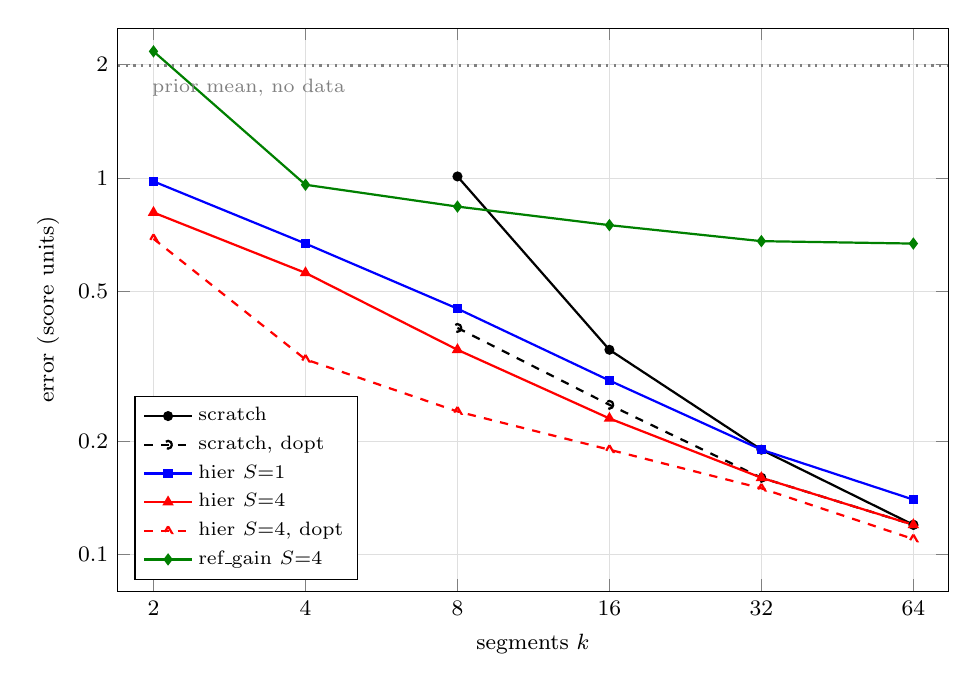
\begin{tikzpicture}
\begin{loglogaxis}[
  width=\columnwidth, height=0.72\columnwidth,
  xlabel={segments $k$}, ylabel={error (score units)},
  xtick={2,4,8,16,32,64}, xticklabels={2,4,8,16,32,64},
  ytick={0.1,0.2,0.5,1,2}, yticklabels={0.1,0.2,0.5,1,2},
  ymin=0.08, ymax=2.5, xmin=1.7, xmax=75,
  legend style={font=\scriptsize, at={(0.02,0.02)}, anchor=south west, cells={anchor=west}},
  grid=major, grid style={gray!25}, tick label style={font=\footnotesize}, label style={font=\footnotesize},
]
\addplot[black, thick, mark=*, mark size=1.4] coordinates {(8,1.01) (16,0.35) (32,0.19) (64,0.12)};
\addlegendentry{scratch}
\addplot[black, thick, dashed, mark=o, mark size=1.4] coordinates {(8,0.40) (16,0.25) (32,0.16) (64,0.12)};
\addlegendentry{scratch, dopt}
\addplot[blue, thick, mark=square*, mark size=1.3] coordinates {(2,0.98) (4,0.67) (8,0.45) (16,0.29) (32,0.19) (64,0.14)};
\addlegendentry{hier $S{=}1$}
\addplot[red, thick, mark=triangle*, mark size=1.6] coordinates {(2,0.81) (4,0.56) (8,0.35) (16,0.23) (32,0.16) (64,0.12)};
\addlegendentry{hier $S{=}4$}
\addplot[red, thick, dashed, mark=triangle, mark size=1.6] coordinates {(2,0.69) (4,0.33) (8,0.24) (16,0.19) (32,0.15) (64,0.11)};
\addlegendentry{hier $S{=}4$, dopt}
\addplot[green!50!black, thick, mark=diamond*, mark size=1.6] coordinates {(2,2.17) (4,0.96) (8,0.84) (16,0.75) (32,0.68) (64,0.67)};
\addlegendentry{ref\_gain $S{=}4$}
\addplot[gray, dotted, thick, domain=1.7:75] {0.05};
\addplot[gray, dotted, thick, domain=1.7:75] {1.99};
\node[gray, font=\scriptsize, anchor=south west] at (axis cs:1.9,0.052) {full grid};
\node[gray, font=\scriptsize, anchor=north west] at (axis cs:1.9,1.95) {prior mean, no data};
\end{loglogaxis}
\end{tikzpicture}

\caption{Simulation, spread 1: few-shot error against the number of segments \(k\) (median over held-out robots and subsets). Solid: random segments; dashed: D-optimal segments. The full-grid fit (405 segments) scores 0.05.}
\label{fig:sim-fewshot}
\end{figure}

\begin{table*}[t]
\caption{Simulation, spread 1: few-shot error (score units, median over held-out robots and subsets) against the number of segments \(k\). \texttt{scratch}: fit on the \(k\) segments alone; \texttt{hier} \(S\): MAP fit under a prior from \(S\) robots; \texttt{ref\_gain}: affine correction of the prior mean; \texttt{dopt}: D-optimal instead of random segments. ``--'': not fittable.}
\label{tab:2}
\centering\footnotesize
\begin{tabular}{lcccccccc}
\toprule
\(k\) & scratch & hier S=1 & hier S=2 & hier S=4 & ref\_gain S=4 & scratch, dopt & hier S=1, dopt & hier S=4, dopt \\
\midrule
2 & -- & 0.98 & 0.82 & 0.81 & 2.17 & -- & 0.91 & 0.69 \\
4 & -- & 0.67 & 0.56 & 0.56 & 0.96 & -- & 0.39 & 0.33 \\
8 & 1.01 & 0.45 & 0.35 & 0.35 & 0.84 & 0.40 & 0.31 & 0.24 \\
16 & 0.35 & 0.29 & 0.25 & 0.23 & 0.75 & 0.25 & 0.22 & 0.19 \\
32 & 0.19 & 0.19 & 0.17 & 0.16 & 0.68 & 0.16 & 0.16 & 0.15 \\
64 & 0.12 & 0.14 & 0.14 & 0.12 & 0.67 & 0.12 & 0.12 & 0.11 \\
\bottomrule
\end{tabular}
\end{table*}


In this synthetic population the prior pays below about 32 segments: at
\(k = 8\) the MAP fit with a four-robot prior scores 0.35 against 1.01
for fitting from scratch with random cells (2.9×) and 0.24 against 0.40
with designed ones (1.7×), and fitting from scratch is not possible
below \(k = 8\) at all; at \(k = 16\) the margin is 1.3--1.5 and by
\(k = 32\) it is gone. D-optimal cells roughly halve the segments needed
at small \(k\): eight designed segments with a four-robot prior match
sixteen random ones. The master/slave baseline plateaus at 0.6--0.9
because an affine correction of a reference map cannot absorb
differences in dead zone and exponent. Sixteen designed segments, about
two minutes of driving, leave an error of 0.19 score units, i.e. 0.95
mm/s and 0.019 rad/s, which is 16 \% of the between-robot spread in
\(u_1\) and 6 \% in \(\omega\), and below the 3 mm/s and 0.05 rad/s
noise of a single segment. A budget of ten minutes, about 75 segments at
the protocol's 8 s per segment, would therefore be generous if real
robots followed the model family; whether they do is what the full grids
of phase B test. The 95 \% intervals of the MAP fit cover the true mean
twist 84--95 \% of the time at \(k \ge 4\) (the floor heuristics are
slightly narrow) and 99--100 \% at \(k = 0\) (the prior is wide).

\subsection{How many calibrated
robots?}\label{sec:sim-power}

Repeating the study over eight simulated populations for fleets of
\(N = 4\), 6 and 8 fully calibrated robots and spreads 0.3, 1 and 3
(Table~\ref{tab:3}) separates the fleet size \(N\) from the prior size
\(S\). The fleet size sets how well the between-robot spread is
\emph{known}: the 10--90 \% band of the estimated robot SD of \(\omega\),
relative to the population value, spans roughly 0.6--1.1 at four robots
and 0.7--1.2 at eight. The expected narrowing of a standard deviation's
sampling error with \(N\), \(\approx 1/\sqrt{2(N-1)}\), is not resolved
by eight populations per cell, so the sweep says that four to eight
full grids leave the spread uncertain by roughly a quarter and no more
than that. The fleet size barely changes how well a \emph{new} robot is
calibrated: at \(k = 16\) a prior from \(S = N-1\) robots gives
0.20--0.29 at every spread except the largest with four robots (0.32),
and a one-robot prior 0.25--0.41; the larger prior lowers the \(k = 16\)
error by 0.02--0.09 in every row, while at \(k = 4\) it helps with six
or eight robots at the two larger spreads and not with four. If real
robots behaved like this population, five or six full grids would be a
reasonable phase B and more would buy a tighter spread estimate rather
than a better few-shot curve; the sample sizes Dechent et al.
\cite{dechent2021samplesize} derive for cell-to-cell variability of
batteries (9--13 cells for one- to three-parameter models) likewise
concern the spread rather than the next unit.

\begin{table*}[t]
\caption{Simulation: sweep over spread and fleet size \(N\), medians over eight populations; the SD ratio is the estimated over the population's between-robot SD of \(\omega\) with its 10--90 \% band. Few-shot scores (score units) for random segments, one subset per robot; \texttt{hier} \(S\): prior from \(S\) robots; \texttt{scratch}: fit on the segments alone; full: all 405 segments.}
\label{tab:3}
\centering\footnotesize
\begin{tabular}{lcccccc}
\toprule
spread & \(N\) & SD ratio & hier S=1, \(k\)=4 / 16 & hier S=N−1, \(k\)=4 / 16 & scratch \(k\)=16 & full \\
\midrule
0.3 & 4 & 0.87 {[}0.61, 1.09{]} & 0.58 / 0.26 & 0.53 / 0.22 & 0.48 & 0.06 \\
0.3 & 6 & 0.91 {[}0.62, 1.09{]} & 0.56 / 0.25 & 0.46 / 0.21 & 0.35 & 0.05 \\
0.3 & 8 & 0.84 {[}0.66, 1.10{]} & 0.57 / 0.25 & 0.42 / 0.20 & 0.33 & 0.05 \\
1.0 & 4 & 0.91 {[}0.61, 1.12{]} & 0.74 / 0.28 & 0.74 / 0.25 & 0.41 & 0.06 \\
1.0 & 6 & 0.95 {[}0.62, 1.12{]} & 0.65 / 0.27 & 0.65 / 0.23 & 0.40 & 0.05 \\
1.0 & 8 & 0.83 {[}0.68, 1.18{]} & 0.66 / 0.27 & 0.55 / 0.24 & 0.34 & 0.05 \\
3.0 & 4 & 0.97 {[}0.58, 1.26{]} & 1.20 / 0.41 & 1.33 / 0.32 & 0.51 & 0.05 \\
3.0 & 6 & 0.90 {[}0.55, 1.35{]} & 1.14 / 0.37 & 0.92 / 0.28 & 0.42 & 0.05 \\
3.0 & 8 & 0.81 {[}0.70, 1.28{]} & 1.32 / 0.36 & 0.91 / 0.29 & 0.37 & 0.05 \\
\bottomrule
\end{tabular}
\end{table*}

\section{Hardware results}\label{sec:hardware-results}

\hw{this section is a skeleton: each slot names the number or figure it
waits for; phase A fills \S\ref{sec:hw-map}, phase B
\S\ref{sec:hw-variability}, phase C \S\ref{sec:hw-fewshot} and
\S\ref{sec:hw-same}}

\subsection{The map of robot \#1}\label{sec:hw-map}

Fig.~\ref{fig:map} shows \(u_1\) and \(\omega\) over the \((L,R)\) grid
with \hw{n} replicates per cell, measured over \hw{D} days. Grouped
cross-validation (Table~\ref{tab:hw-cv}) selects the \hw{lin / int /
cor / bat} variant with an error of \hw{x} cm/s in \(u_1\) and \hw{y}
rad/s in \(\omega\), against \hw{x, y} for the best polynomial, \hw{x,
y} for the Gaussian process and \hw{x, y} for the neural network. The
fitted dead zones are \hw{p0L, p0R} and the exponents \hw{gammaL,
gammaR}; the interaction term \(f_L f_R\) \hw{is / is not} supported by
the data. At the top of the grid the speed \hw{stays monotone / reverses
at power P}. The 40 kHz PWM mode \hw{changes only the gain by G \% /
changes the dead zone and exponent}. The mean centre-of-rotation offset
is \(\bar d = \) \hw{d} mm (bootstrap 95 \% interval \hw{lo--hi}); the
step responses \hw{do / do not} separate the clockwise and
counter-clockwise offsets. The lag is \(\tau = \) \hw{tau} s with a dead
time of \hw{t0} s, the heading diffusion \(D_r = \) \hw{Dr} rad\(^2\)/s
\hw{Brownian / OU}. Parameter standard deviations are within \hw{factor}
of the Cramér--Rao bound. Over three days the map drifted by \hw{drift}
in gain and \hw{drift} in dead zone, and the \texttt{bat} term accounts
for \hw{share} of it.

\begin{figure}[t]
\centering
\fbox{\parbox[c][5cm][c]{0.95\columnwidth}{\centering \hw{Fig.~1: \(u_1\) and \(\omega\) over the grid, replicates, fitted map, top-of-grid check}}}
\caption{Robot \#1's forward map. \hw{caption}}
\label{fig:map}
\end{figure}

\begin{table}[t]
\caption{Grouped cross-validation on robot \#1 (RMSE on held-out cells). \hw{fill}}
\label{tab:hw-cv}
\centering\footnotesize
\begin{tabular}{lcc}
\toprule
model & \(u_1\) [cm/s] & \(\omega\) [rad/s] \\
\midrule
\texttt{lin} & -- & -- \\
\texttt{int} & -- & -- \\
\texttt{cor} & -- & -- \\
\texttt{bat} & -- & -- \\
polynomial (plane / quadratic / cubic) & -- & -- \\
Gaussian process & -- & -- \\
neural network & -- & -- \\
\bottomrule
\end{tabular}
\end{table}

\subsection{How different are \hw{N} robots}\label{sec:hw-variability}

Fig.~\ref{fig:variance} and Table~\ref{tab:hw-variance} give the robot
/ day / segment standard deviations per output over \hw{N} robots and
\hw{D} days. The robot component is \hw{x} cm/s in \(u_1\) and \hw{y}
rad/s in \(\omega\), \hw{r} times the segment noise and \hw{r} times
the day component; the fractions are \hw{robot / day / segment}. The
between-robot differences are \hw{dominated by gain / by dead zone /
spread across parameters} (Fig.~\ref{fig:variance}, right), and the
fitted population prior has \hw{SDs per parameter}.

\begin{figure}[t]
\centering
\fbox{\parbox[c][5cm][c]{0.95\columnwidth}{\centering \hw{Fig.~2: variance components per output; per-parameter spread of the fitted maps; the population prior}}}
\caption{Variability across \hw{N} robots and \hw{D} days. \hw{caption}}
\label{fig:variance}
\end{figure}

\begin{table}[t]
\caption{Measured robot, day and segment standard deviations (compare Table~\ref{tab:1}). \hw{fill}}
\label{tab:hw-variance}
\centering\footnotesize
\begin{tabular}{lcccc}
\toprule
output & robot SD & day SD & segment SD & fractions \\
\midrule
\(u_1\) [m/s] & -- & -- & -- & -- \\
\(u_2\) [m/s] & -- & -- & -- & -- \\
\(\omega\) [rad/s] & -- & -- & -- & -- \\
\bottomrule
\end{tabular}
\end{table}

\subsection{Calibrating a new robot}\label{sec:hw-fewshot}

Fig.~\ref{fig:fewshot} and Table~\ref{tab:hw-fewshot} give the
leave-one-robot-out error against the number of segments \(k\), scored
on each robot's measured segments outside the chosen subset. With a
prior from \hw{S = N-1} robots and \hw{k} designed segments (about \hw{t}
minutes of driving) the error reaches \hw{x} noise units, \hw{r} times
better than fitting from scratch at the same budget and \hw{r} times
better than the master/slave standardisation, which plateaus at \hw{x}.
The Klingner-style black-box search reaches \hw{x} after \hw{k}
segments. A prior from one robot \hw{is / is not} enough beyond \(k =
\) \hw{k}. The 95 \% predictive intervals cover the held-out segments
\hw{c} of the time. \hw{if any robot falls outside the model family,
say which and how it showed}

\begin{figure}[t]
\centering
\fbox{\parbox[c][5cm][c]{0.95\columnwidth}{\centering \hw{Fig.~3: error vs \(k\), random vs designed, priors from 1 / 2 / 4 robots, baselines, coverage}}}
\caption{Few-shot calibration of held-out robots. \hw{caption}}
\label{fig:fewshot}
\end{figure}

\begin{table*}[t]
\caption{Measured few-shot error against \(k\), median over held-out robots (compare Table~\ref{tab:2}). \hw{fill}}
\label{tab:hw-fewshot}
\centering\footnotesize
\begin{tabular}{lcccccccc}
\toprule
\(k\) & scratch & black-box & ref\_gain & hier S=1 & hier S=2 & hier S=4 & hier S=1, dopt & hier S=4, dopt \\
\midrule
2 & -- & -- & -- & -- & -- & -- & -- & -- \\
4 & -- & -- & -- & -- & -- & -- & -- & -- \\
8 & -- & -- & -- & -- & -- & -- & -- & -- \\
16 & -- & -- & -- & -- & -- & -- & -- & -- \\
32 & -- & -- & -- & -- & -- & -- & -- & -- \\
64 & -- & -- & -- & -- & -- & -- & -- & -- \\
\bottomrule
\end{tabular}
\end{table*}

\subsection{Same command, same motion}\label{sec:hw-same}

Fig.~\ref{fig:same} shows the achieved \((v,\omega)\) when every robot
is commanded the same targets through its own inverse map, on the
intersection of the feasible sets. Before calibration (one shared map)
the across-robot spread is \hw{x} cm/s and \hw{y} rad/s; after
per-robot calibration it is \hw{x} cm/s and \hw{y} rad/s, \hw{r} times
the segment noise. \hw{whether the residual spread is drift, model
error or noise}

\begin{figure}[t]
\centering
\fbox{\parbox[c][5cm][c]{0.95\columnwidth}{\centering \hw{Fig.~4: achieved vs commanded \((v,\omega)\) per robot, before and after calibration}}}
\caption{Same commanded velocity on all robots. \hw{caption}}
\label{fig:same}
\end{figure}

\section{Discussion}\label{sec:discussion}

\hw{this section argues from the simulation and the literature only;
rewrite from the measurements}

\textbf{What the simulation can and cannot say.} In the simulation the
prior's value is concentrated below 32 segments, and a one-robot prior
is within 30 \% of a four-robot prior from eight segments on, because
the population was drawn from the model family. On real robots the risk
is misspecification: a robot whose dead zone or reversal point falls
outside the family would be pulled towards the prior and look calibrated
when it is not. The predictive-interval coverage and the held-out
measured segments detect this; the full grids of phase B locate it.

\textbf{Drift.} The day component of the decomposition, the battery term
of the \texttt{bat} variant and the three-day repeat on robot \#1 are
designed to quantify what the Kilobot literature reports qualitatively
\cite{raoufi2023individuality, rubenstein2014kilobot}. If drift turns
out to be a sizeable fraction of the robot component, a recursive
least-squares update of the thirteen parameters during operation,
keyed by chip serial, is one extension
\cite{martinelli2007selfcalibration, roy1999selfcalibration}.

\textbf{Outlook: setting heterogeneity.} If the measured robot
component dominates the decomposition, calibration could remove it, and
the same machinery could set a chosen heterogeneity: Giomi et al.
\cite{giomi2013bristlebots} show that a per-robot spin-to-walk ratio
selects the collective state, and Siebers et al.
\cite{siebers2023disorder} exploit disorder deliberately. Whether a
calibrated GRASPion fleet can serve as an active-matter experiment with
a controlled disorder parameter depends on the measured decomposition.

\textbf{Open questions the data will decide.} Whether the two motors add
linearly, as Notomista et al. \cite{notomista2019brushbot} derive, or
interact; whether transient data identify the CW / CCW split that
steady-state data cannot; whether the PWM frequency changes the map's
shape or only its gain; and whether the onboard magnetometer, once its
hard-iron offset \cite{vasconcelos2011magnetometer} and the offset
\(b(L,R)\) that the running motors induce at each drive level are
mapped, can carry the yaw-rate part
of recalibration without a camera.

\section{Limitations}\label{sec:limitations}

\hw{rewrite once the campaign is done} No hardware result exists yet, so
the abstract, discussion and conclusion contain no measured claim about
GRASPion; the simulation cannot
show model misspecification, lag, battery dependence or the high-drive
reversal; segment noise is assumed constant over the grid, whereas
Swarmodroid reports dispersion growing with drive
\cite{dmitriev2023swarmodroid}; the prior drops cross-block covariance;
the D-optimal design is local to the prior mean; the literature search
was not systematic \hw{remove before submission: bib entries marked
abstract only or verify must be read in full}. The robot, the 7×7 tables
and the twin's kinematic model are the GRASP lab's, and the reanalysis
of §\ref{sec:lab-tables} is of their public code.

\section{Conclusion}\label{sec:conclusion}

Three things are established without hardware: that steady-state data
identify the mean but not the split of a two-motor vibration robot's
centre-of-rotation offset; that on the lab's published tables a
dead-zone power law is as accurate as low-order polynomials and adds a
closed-form inverse and a feasible set; and that the proposed few-shot
calibration, run on a synthetic population drawn from the model family,
recovers the injected variability and reduces a new robot's error with
each added segment as intended. The three questions of the introduction, what the simplest
adequate model is, how different nominally identical GRASPions are, and
how few measurements a new one needs, are empirical, and this draft does
not answer them. \hw{replace with the measured answers to the three
questions, including which kill criterion, if any, applied}


\bibliographystyle{IEEEtran}
\bibliography{refs}

\end{document}
